\documentclass[12pt,a4paper]{article}

% ─── Encoding & Fonts ───
\usepackage[utf8]{inputenc}
\usepackage[T1]{fontenc}
\usepackage{lmodern}

% ─── Page Layout ───
\usepackage[top=2.5cm,bottom=2.5cm,left=3cm,right=2.5cm]{geometry}
\usepackage{setspace}
\onehalfspacing

% ─── Section Formatting ───
\usepackage{titlesec}
\titleformat{\section}{\large\bfseries}{\thesection.}{0.5em}{}
\titleformat{\subsection}{\normalsize\bfseries}{\thesubsection}{0.5em}{}

% ─── Lists ───
\usepackage{enumitem}

% ─── Tables ───
\usepackage{booktabs}
\usepackage{longtable}
\usepackage{tabularx}

% ─── Graphics & Colours ───
\usepackage{graphicx}
\usepackage[dvipsnames]{xcolor}
\usepackage{tikz}
\usetikzlibrary{
  arrows.meta,
  positioning,
  shapes.multipart,
  shapes.geometric,
  fit,
  calc,
  backgrounds,
  decorations.pathreplacing
}

% ─── Floats & Captions ───
\usepackage{float}
\usepackage{caption}
\captionsetup{font=small,labelfont=bf,skip=8pt}

% ─── References ───
\usepackage[round,authoryear]{natbib}
\bibliographystyle{apalike}

% ─── Hyperlinks ───
\usepackage[colorlinks=true,linkcolor=MidnightBlue,citecolor=MidnightBlue,urlcolor=MidnightBlue]{hyperref}

% ─── Maths ───
\usepackage{amsmath,amssymb}

% ─── Avoid widows/orphans ───
\widowpenalty=10000
\clubpenalty=10000

% ─── Custom colours for TikZ ───
\definecolor{phaseblue}{HTML}{2C3E50}
\definecolor{trackgreen}{HTML}{27AE60}
\definecolor{trackorange}{HTML}{E67E22}
\definecolor{fusionpurple}{HTML}{8E44AD}
\definecolor{evalred}{HTML}{C0392B}
\definecolor{lightbg}{HTML}{ECF0F1}
\definecolor{safetyyellow}{HTML}{F39C12}

\begin{document}

% ─── TITLE PAGE ───
\begin{titlepage}
\centering
\vspace*{1cm}

{\Large\bfseries Jomo Kenyatta University of Agriculture and Technology}\\[0.3cm]
{\large School of Computing and Information Technology}\\[0.3cm]
{\large Department of Computing}\\[1.5cm]

{\LARGE\bfseries A Causal Evaluation of Culturally Adaptive AI\\[0.3cm]
as Relational Scaffolding for Loneliness Intervention}\\[2cm]

{\large A Research Proposal Submitted in Partial Fulfilment\\
of the Requirements for the Degree of\\[0.3cm]
\textbf{Master of Science in Artificial Intelligence}}\\[2cm]

{\large\textbf{Student:} Kinyua Seaman}\\[0.5cm]
{\large\textbf{Supervisors:} Dr.\ Lawrence Nderu \quad Dr.\ Raphael Wanjiku}\\[2cm]

{\large 1st June 2026}

\vfill
\end{titlepage}

% ─── ABSTRACT ───
\section*{Abstract}
\addcontentsline{toc}{section}{Abstract}

Digital mental health interventions show considerable promise for tackling the global loneliness epidemic, yet conversational AI systems consistently underserve non-Western populations. Built on Western individualistic psychiatric frameworks, these models carry severe epistemic bias: they routinely misread communal expressions of psychological distress. For instance, when a user in Nairobi describes \textit{kufikiria sana} (thinking too much), standard models tend to pathologise this as clinical anxiety rather than recognising the communal disruption it signifies. Furthermore, many commercial platforms foster what may be termed the ``Companionship Paradox,'' functioning as synthetic replacements for human connection instead of temporary therapeutic scaffolding aimed at restoring real-world relationships.

Network analysis of adolescent psychosocial functioning in Kenya identifies loneliness as the most central psychological variable, bridging depressive symptoms and diminished well-being through gender-contingent pathways: family support proves more central for girls, whereas peer support plays a larger role for boys \citep{Ndetei2025}. This research proposes a culturally adaptive conversational AI built on a dual-track Retrieval-Augmented Generation (RAG) pipeline that grounds the intervention in both East African cultural knowledge and evidence-based Cognitive Behavioural Therapy (CBT). The system translates standard behavioural activation protocols into culturally resonant metaphors while prioritising relational well-being and community reintegration over isolated symptom management.

To establish clinical efficacy, this study employs a rigorous causal inference framework. Current human-computer interaction (HCI) research suffers from over-reliance on correlational engagement metrics. By deploying structural causal models alongside deep graph learning techniques, this work systematically compares culturally adapted outputs against generic baseline responses, isolating the therapeutic ``outcome delta.'' This methodological advance addresses a critical question: does algorithmic cultural adaptation directly and causally drive longitudinal loneliness reduction? The resulting open-source framework will offer a scalable blueprint for ethical digital health infrastructure serving diverse populations globally.

% ─── SECTION 1 ───
\section{Problem Formulation and Research Objectives}

\subsection{Statement of the Problem and Research Gaps}

The rapid integration of generative AI into digital mental health has created new possibilities for scalable loneliness intervention. However, deployment in resource-constrained, non-Western settings reveals critical structural and methodological shortcomings. Three primary research gaps constrain current paradigms:

\paragraph{Cultural Inflexibility and Epistemic Bias.}
Existing AI companions fundamentally lack adaptation for non-Western linguistic and social contexts. Foundation models, trained predominantly on Western corpora, misinterpret communal idioms of distress with alarming regularity. Systematic reviews of conversational agents for mental health have found widespread reliance on Western-developed scales, minimal cultural adaptation, a predominance of small and short-duration studies, and weak links between automated performance metrics and actual user well-being \citep{EvalSysReview2026}. Ethnographic research in urban Kenya has documented \textit{kufikiria sana} as a powerful idiom that reflects both individual suffering and social anxieties, embedding psychological distress firmly within relational contexts \citep{Mendenhall2019}. These findings demand intervention designs that validate, rather than pathologise, culturally specific expressions.

\paragraph{The Absence of Relational Scaffolding.}
Most commercial conversational agents optimise for prolonged user engagement rather than clinical recovery. Recent longitudinal research reveals a troubling paradox: AI companions provide unconditional, unflagging support that attracts socially struggling individuals, yet extended use may erode well-being and impair the capacity to navigate real-world relationships \citep{Jovanovic2026}. Investigations into the relationship between depression and conversational AI use among college students have found that depression positively associates with AI companion use, with loneliness mediating this link \citep{DepressionAI2025}. A critical gap remains in designing systems that deliver evidence-based therapeutic responses while actively guiding users toward renewed human community engagement.

\paragraph{The HCI Evaluation Deficit.}
Evaluations of mental health chatbots rely heavily on weak, correlational data. Researchers frequently fail to isolate precise mechanisms of clinical change. Systematic reviews and meta-analyses of generative AI chatbots for mental health have underscored the urgent need for large-scale, multicultural trials with culturally adapted AI to optimise safety, efficacy, and equity \citep{Viduani2025}. A rigorous causal inference framework is needed to quantify the true impact of localised conversational interventions.

\subsection{Aim of the Study}

The overarching aim is to design, implement, and evaluate personalised AI conversations that measurably reduce loneliness. This study will engineer a culturally adaptive generative pipeline using Microsoft Azure OpenAI and a RAG architecture. By grounding the model in both evidence-based CBT and localised cultural knowledge, the system will translate standard therapeutic strategies into culturally resonant dialogue. Through structural comparison of localised interventions against generic baseline responses using causal models, this research will isolate the therapeutic ``outcome delta,'' demonstrating the clinical necessity of deep algorithmic cultural adaptation.

\subsection{Research Questions}

\paragraph{Primary Research Question:}
How can a personalised, culturally adaptive conversational AI companion be designed, fine-tuned, and rigorously evaluated to deliver evidence-based interventions that measurably reduce loneliness in target populations?

\paragraph{Secondary Research Questions:}
\begin{enumerate}[label=\textbf{RQ\arabic*:},leftmargin=2cm]
  \setcounter{enumi}{1}
  \item[\textbf{RQ2a}] \textbf{(Architectural):} How does anchoring generative models within a localised RAG pipeline mitigate the epistemic bias and clinical hallucination present in standard Western-trained models?
  \item[\textbf{RQ2b}] \textbf{(Evaluative):} What is the quantifiable, causal impact of algorithmic cultural adaptation on longitudinal loneliness reduction when structural causal models compare culturally tailored responses against generic therapeutic baselines?
\end{enumerate}

% ─── SECTION 2 ───
\section{Literature Review}

Integrating large language models (LLMs) into digital mental health creates opportunities for scalable loneliness support. However, deploying these systems in non-Western environments exposes significant limitations. This review synthesises recent work on conversational agents, epistemic bias, cultural adaptation, and causal evaluation.

\subsection{Efficacy and Limitations of Generic Conversational Agents}

Rule-based and generative AI chatbots have demonstrated capacity for delivering structured psycho-education and CBT prompting. Meta-analytic evidence suggests that generative AI mental health chatbots outperform rule-based systems in reducing mental health symptoms \citep{Viduani2025}. Evaluations of LLMs delivering CBT indicate that, while these models generate plausible CBT-like dialogues, they remain limited in conveying empathy and maintaining therapeutic consistency \citep{Bedi2026}. Comparative studies of generalist versus specialised models in RAG-based mental health dialogue have found that generalist reasoners surpass domain-specific fine-tuned models in empathy, suggesting that reasoning capability matters more than domain-specific vocabulary \citep{Kafi2026}.

Despite these technical capabilities, the clinical value of purely generative models remains contested. A cross-cultural study spanning 4,641 participants across seven countries revealed mixed outcomes: greater short-term comfort co-occurred with increases in language about loneliness, depression, and suicidal ideation over time \citep{AmatLefort2026}. This ``Companionship Paradox'' suggests that highly responsive LLMs risk functioning as ``relational mirages,'' where sustained reliance on AI for emotional regulation can paradoxically deepen offline isolation.

\subsection{Cultural Adaptation and Epistemic Constraints}

Deploying conversational interventions in Sub-Saharan Africa exposes severe epistemic biases embedded in foundation models. Research on multilingual depression classification has shown that model accuracy varies markedly across languages, with demographic biases affecting performance in non-English settings. \citet{Xie2025} developed a novel approach for dynamic cultural adaptation of LLM-based mental health agents through context engineering for Chinese American caregivers. The culturally adapted agent produced significant improvements in near-term emotional well-being and received higher ratings for cultural competence and therapeutic alliance relative to a non-adapted baseline.

This line of inquiry has extended to additional populations. Researchers developed Molhim, a culturally adapted multimodal conversational AI platform for PTSD screening, demonstrating the feasibility of structured clinical dialogue across cultural boundaries \citep{Ozel2026}. An Ubuntu-guided LLM framework integrating CBT with the African philosophy of Ubuntu has been proposed as a proof of concept for culturally sensitive AI mental health dialogue \citep{Ubuntu2026}. Particularly relevant to East Africa, the Shamiri Institute has launched shamiriAI, an AI-powered mental health platform for youth across Africa, building on a community-based model that has reached over 185,000 young people in Kenya through school-based interventions led by trained peer providers \citep{Shamiri2025}.

\subsection{Idioms of Distress in East African Contexts}

Psychological distress in East African populations often manifests through culturally specific idioms that do not align with Western diagnostic categories. Analysis of 100 life-history narrative interviews among patients at a public hospital in Nairobi revealed that \textit{kufikiria sana} emerged organically as a salient cultural idiom that functions both as a standalone expression and as a marker of other psychological distress \citep{Mendenhall2019}. This ethnopsychology integrates local (traditional) and biomedical frameworks that are both distinct and overlapping in their symptomatology and experiential dimensions.

Network-based analysis of adolescent psychosocial functioning in Kenya has identified loneliness as the most central psychological variable, directly bridging depressive symptoms and diminished well-being \citep{Ndetei2025}. Family support proves more central for girls, whereas peer support plays a greater role for boys, underscoring the need for contextually and gender-sensitive interventions. The Swahili expression \textit{ipo siku} (there will come a day) and the colloquial term ``Njaanuary'' reflect local coping mechanisms and cultural understandings of hardship that must inform any culturally competent intervention.

\subsection{Causal Inference in Mental Health AI}

Current evaluation of HCI in mental health relies largely on correlational longitudinal studies. Recent methodological advances offer pathways to address this limitation. Causal graph neural networks have been proposed as a framework for integrating causal inference with graph-based deep learning, enabling a shift from pattern recognition to causal reasoning in healthcare AI \citep{Mesinovic2026}. InsightFlow demonstrated that LLMs can produce clinically meaningful causal graphs from patient-therapist dialogues, achieving structural similarity comparable to inter-annotator agreement \citep{Gupta2026}.

\citet{Wang2025} identified daily-living features related to loneliness using causal machine learning, establishing that social interactions, physical activity, sleep, and cardiac features have a causal influence on loneliness. A Bayesian decision-theoretic framework for ranking digital mental health interventions based on individual presentation has also been proposed \citep{CausalAIRec2025}. Nevertheless, no existing study has extended causal inference approaches to evaluate cultural adaptation in conversational AI.

\subsection{Research Gap Synthesis}

The reviewed literature reveals a clear gap: while RAG-based cultural adaptation has shown promise in Chinese American and other non-Western contexts, and while East African idioms of distress have been extensively documented, no study has combined these insights to develop a culturally adapted conversational AI for Kenyan youth. Furthermore, no research has employed causal inference frameworks to isolate the specific effect of algorithmic cultural adaptation on loneliness reduction. This research directly addresses both gaps.

% ─── SECTION 3 ───
\section{Methodology}

This research follows a four-phase sequential pipeline designed to capture signals, translate culture, generate relational scaffolding, and causally evaluate outcomes over a six-month period. Phases overlap where feasible to maximise efficiency.

\subsection{Phase 1: Signal Ingestion and Clinical Governance (Month 1)}

The intervention begins with system setup and safety framework implementation. The pipeline continuously ingests detection confidence scores from the edge deployment layer. When a user's state crosses a predefined clinical threshold, the active intervention workflow triggers. Safety remains the absolute priority throughout. Every text input passes through strict content safety filters (Azure AI Content Safety) before processing. If the system detects severe distress or self-harm indicators, it immediately bypasses the generative engine and activates a hard-coded clinical escalation protocol.

\subsection{Phase 2: Dual-Track Retrieval-Augmented Generation (Months 1--2)}

This phase addresses the epistemic bias inherent in global language models through a dual-track RAG pipeline constructed via Azure AI Search:

\begin{description}[style=nextline]
  \item[Track A (Clinical Grounding)]
  Queries a curated repository of CBT protocols, behavioural activation strategies, and evidence-based psycho-educational materials validated for adolescent populations.

  \item[Track B (Cultural Translation)]
  Simultaneously queries a knowledge base of East African idioms of distress (including \textit{kufikiria sana}, \textit{kufa moyo}, \textit{ipo siku}), culturally resonant metaphors, communal coping strategies, and validated cultural responses. This repository draws from published ethnographic research \citep{Mendenhall2019}, clinical expertise from local mental health practitioners, and community-based participatory design.
\end{description}

The pipeline fuses these knowledge streams into a single contextualised data packet. This architecture mirrors successful implementations in mental health dialogue systems, with empirical evidence showing that RAG significantly reduces hallucinations and improves contextual relevance compared to generation-only approaches \citep{Kafi2026}.

\subsection{Phase 3: Generative Formulation for Relational Scaffolding (Months 2--3)}

With context fused, the system proceeds to response formulation. The RAG packet feeds into the generative engine via a dynamic system prompt that explicitly constrains the AI persona to function as relational scaffolding rather than a synthetic companion. The prompt includes:

\begin{itemize}
  \item A directive to prioritise community reintegration over prolonged engagement;
  \item Instructions to employ locally resonant metaphors and communal language registers;
  \item Guidelines for action-oriented suggestions promoting real-world social connection;
  \item Prohibitions against encouraging dependency.
\end{itemize}

The ultimate goal of every generated response is to guide the user toward re-engaging with their physical community.

\subsection{Phase 4: Longitudinal Telemetry and Causal Evaluation (Months 3--6)}

This phase constitutes the core scientific contribution. Rather than relying on weak correlational metrics, evaluation is treated as a rigorous causal inference problem.

\paragraph{Study Design.}
A two-arm randomised controlled trial (RCT) with $N \geq 200$ Kenyan youth participants (aged 14--25). Participants are randomised into:

\begin{itemize}
  \item \textbf{Intervention arm} ($n \geq 100$): Culturally adaptive RAG pipeline with dual-track retrieval.
  \item \textbf{Control arm} ($n \geq 100$): Generic baseline using the same LLM without cultural RAG.
\end{itemize}

\paragraph{Instruments.}
Loneliness is measured at baseline (T0), week 4 (T1), and week 8 (T2) using the Revised UCLA Loneliness Scale (Version 3), which demonstrates high internal consistency (Cronbach's $\alpha$ ranging from .89 to .94) and acceptable test--retest reliability over a one-year period ($r = .73$) \citep{Russell1996}. Secondary measures include therapeutic alliance, engagement duration, and self-reported community reintegration behaviours.

\paragraph{Causal Analysis.}
Structural causal models and deep graph learning techniques are deployed to systematically compare the intervention and control arms. Causal graph neural networks enable integration of causal inference with graph-based deep learning to learn invariant mechanisms rather than spurious correlations \citep{Mesinovic2026}. This approach mathematically isolates the cultural adaptation variable, providing evidence for whether cultural adaptation directly causes a reduction in loneliness scores.

\subsection{Technical Architecture Summary}

Table~\ref{tab:architecture} summarises the key components of the proposed system.

\begin{table}[H]
\centering
\caption{Technical architecture components.}
\label{tab:architecture}
\begin{tabularx}{\textwidth}{lX}
\toprule
\textbf{Component} & \textbf{Implementation} \\
\midrule
Foundation Model & Azure OpenAI GPT-4o \\
Retrieval Engine & Azure AI Search with hybrid retrieval \\
Safety Filter & Azure AI Content Safety \\
Clinical Knowledge Base & Curated CBT protocols, behavioural activation strategies \\
Cultural Knowledge Base & East African idioms, metaphors, communal coping strategies \\
Validation Instrument & UCLA Loneliness Scale (Version 3) \\
Causal Framework & Structural causal models, causal graph neural networks \\
\bottomrule
\end{tabularx}
\end{table}

% ─── ARCHITECTURE DIAGRAM (TikZ) ───
\begin{figure}[H]
\centering
\resizebox{\textwidth}{!}{%
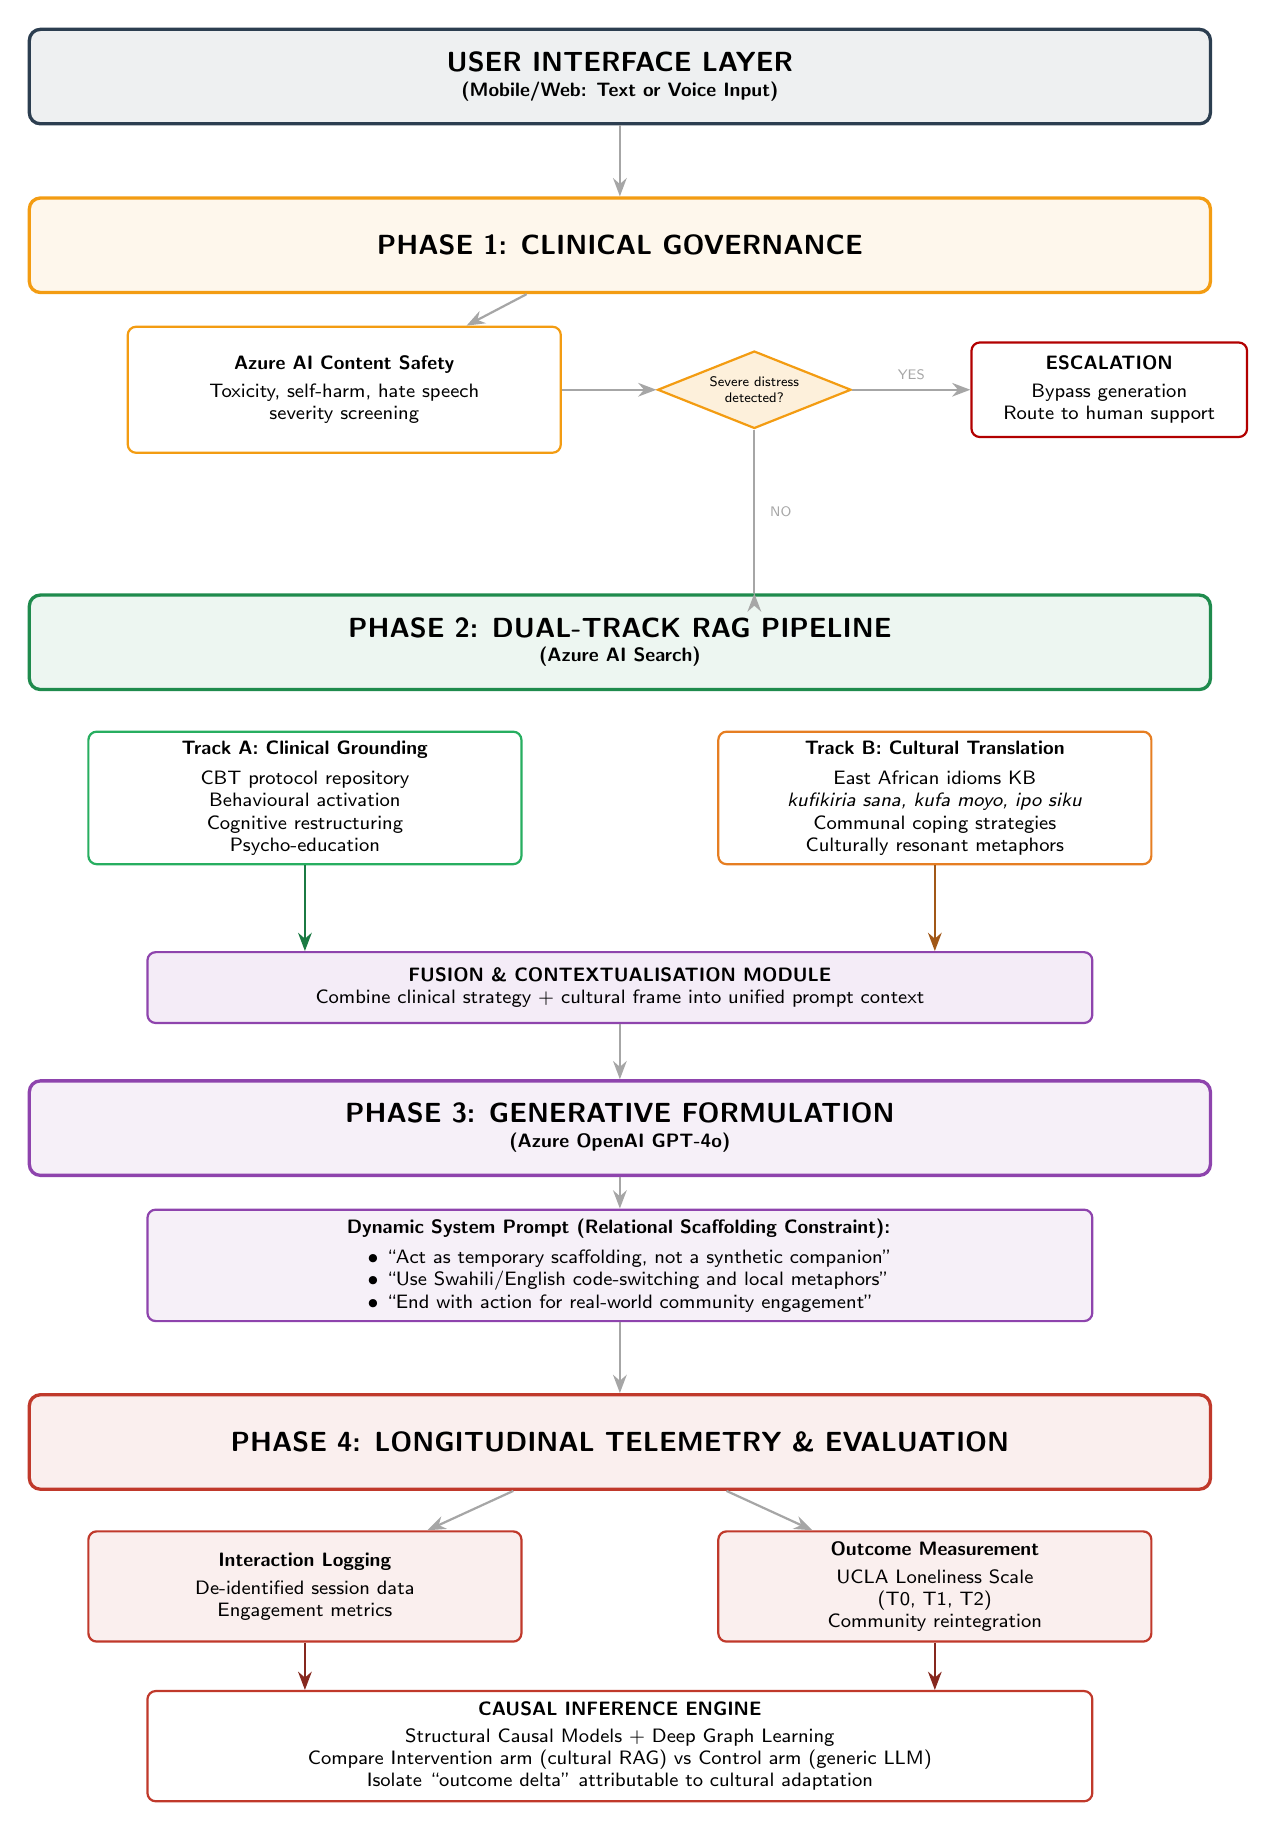
\begin{tikzpicture}[
    >=Stealth,
    node distance=0.8cm,
    % Styles
    phase/.style={
        rectangle, rounded corners=4pt,
        draw=#1, line width=1.2pt,
        fill=#1!8, text=black,
        minimum width=15cm, minimum height=1.2cm,
        font=\sffamily\bfseries\small,
        align=center
    },
    subbox/.style={
        rectangle, rounded corners=3pt,
        draw=#1, line width=0.8pt,
        fill=white, text=black,
        minimum width=5.5cm, minimum height=1.6cm,
        font=\sffamily\scriptsize,
        align=center
    },
    fusionbox/.style={
        rectangle, rounded corners=3pt,
        draw=fusionpurple, line width=0.8pt,
        fill=fusionpurple!10, text=black,
        minimum width=12cm, minimum height=0.9cm,
        font=\sffamily\scriptsize,
        align=center
    },
    promptbox/.style={
        rectangle, rounded corners=3pt,
        draw=fusionpurple, line width=0.8pt,
        fill=fusionpurple!8, text=black,
        minimum width=12cm,
        font=\sffamily\scriptsize,
        align=left
    },
    evalbox/.style={
        rectangle, rounded corners=3pt,
        draw=evalred, line width=0.8pt,
        fill=evalred!8, text=black,
        minimum width=5.5cm, minimum height=1.4cm,
        font=\sffamily\scriptsize,
        align=center
    },
    connector/.style={->, thick, color=gray!70},
    decision/.style={
        diamond, draw=safetyyellow, line width=0.8pt,
        fill=safetyyellow!15,
        font=\sffamily\tiny,
        align=center,
        inner sep=2pt,
        aspect=2.5
    }
]

% ── USER INTERFACE ──
\node[phase=phaseblue] (ui) {\normalsize USER INTERFACE LAYER\\[-2pt]\scriptsize(Mobile/Web: Text or Voice Input)};

% ── PHASE 1: CLINICAL GOVERNANCE ──
\node[phase=safetyyellow, below=0.9cm of ui] (p1label) {\normalsize PHASE 1: CLINICAL GOVERNANCE};

\node[subbox=safetyyellow, below=0.4cm of p1label, xshift=-3.5cm] (safety) {
    \textbf{Azure AI Content Safety}\\[2pt]
    Toxicity, self-harm, hate speech\\
    severity screening
};

\node[decision, right=1.2cm of safety] (decide) {Severe distress\\detected?};

\node[subbox=red!70!black, right=1.5cm of decide, minimum width=3.5cm, minimum height=1.2cm] (escalate) {
    \textbf{ESCALATION}\\[2pt]
    Bypass generation\\
    Route to human support
};

\draw[connector] (ui) -- (p1label);
\draw[connector] (p1label) -- (safety);
\draw[connector] (safety) -- (decide);
\draw[connector] (decide) -- node[above, font=\sffamily\tiny] {YES} (escalate);

% ── PHASE 2: DUAL-TRACK RAG ──
\node[phase=trackgreen!80!black, below=3.8cm of p1label] (p2label) {\normalsize PHASE 2: DUAL-TRACK RAG PIPELINE\\[-2pt]\scriptsize(Azure AI Search)};

\draw[connector] (decide) -- node[right, font=\sffamily\tiny, xshift=2pt] {NO} (decide |- p2label.north) -- (p2label.north -| decide);

\node[subbox=trackgreen, below=0.5cm of p2label, xshift=-4cm] (trackA) {
    \textbf{Track A: Clinical Grounding}\\[3pt]
    CBT protocol repository\\
    Behavioural activation\\
    Cognitive restructuring\\
    Psycho-education
};

\node[subbox=trackorange, below=0.5cm of p2label, xshift=4cm] (trackB) {
    \textbf{Track B: Cultural Translation}\\[3pt]
    East African idioms KB\\
    \textit{kufikiria sana, kufa moyo, ipo siku}\\
    Communal coping strategies\\
    Culturally resonant metaphors
};

\node[fusionbox, below=0.7cm of p2label, yshift=-2.6cm] (fusion) {
    \textbf{FUSION \& CONTEXTUALISATION MODULE}\\
    Combine clinical strategy + cultural frame into unified prompt context
};

\draw[connector, color=trackgreen!70!black] (trackA.south) -- ++(0,-0.3) -| (fusion.north -| trackA);
\draw[connector, color=trackorange!70!black] (trackB.south) -- ++(0,-0.3) -| (fusion.north -| trackB);

% ── PHASE 3: GENERATIVE FORMULATION ──
\node[phase=fusionpurple, below=0.7cm of fusion] (p3label) {\normalsize PHASE 3: GENERATIVE FORMULATION\\[-2pt]\scriptsize(Azure OpenAI GPT-4o)};

\node[promptbox, below=0.4cm of p3label] (prompt) {
    \textbf{Dynamic System Prompt (Relational Scaffolding Constraint):}\\[3pt]
    \quad$\bullet$ ``Act as temporary scaffolding, not a synthetic companion''\\
    \quad$\bullet$ ``Use Swahili/English code-switching and local metaphors''\\
    \quad$\bullet$ ``End with action for real-world community engagement''
};

\draw[connector] (fusion) -- (p3label);
\draw[connector] (p3label) -- (prompt);

% ── PHASE 4: EVALUATION ──
\node[phase=evalred, below=0.9cm of prompt] (p4label) {\normalsize PHASE 4: LONGITUDINAL TELEMETRY \& EVALUATION};

\node[evalbox, below=0.5cm of p4label, xshift=-4cm] (logging) {
    \textbf{Interaction Logging}\\[2pt]
    De-identified session data\\
    Engagement metrics
};

\node[evalbox, below=0.5cm of p4label, xshift=4cm] (instruments) {
    \textbf{Outcome Measurement}\\[2pt]
    UCLA Loneliness Scale\\
    (T0, T1, T2)\\
    Community reintegration
};

\node[subbox=evalred, below=0.6cm of logging, xshift=4cm, minimum width=12cm, minimum height=1.4cm] (causal) {
    \textbf{CAUSAL INFERENCE ENGINE}\\[2pt]
    Structural Causal Models + Deep Graph Learning\\
    Compare Intervention arm (cultural RAG) vs Control arm (generic LLM)\\
    Isolate ``outcome delta'' attributable to cultural adaptation
};

\draw[connector] (prompt) -- (p4label);
\draw[connector] (p4label) -- (logging);
\draw[connector] (p4label) -- (instruments);
\draw[connector, color=evalred!70!black] (logging.south) -- ++(0,-0.25) -| (causal.north -| logging);
\draw[connector, color=evalred!70!black] (instruments.south) -- ++(0,-0.25) -| (causal.north -| instruments);

\end{tikzpicture}
}%
\caption{Schematic diagram of the proposed dual-track RAG architecture for culturally adaptive loneliness intervention. The pipeline comprises four sequential phases: (1)~Clinical Governance with safety filtering; (2)~Dual-Track RAG retrieval from CBT protocols (Track~A) and East African cultural knowledge bases (Track~B); (3)~Generative formulation constrained by relational scaffolding prompts; (4)~Longitudinal evaluation using validated psychometric instruments and causal inference models to isolate the effect of cultural adaptation.}
\label{fig:architecture}
\end{figure}

% ─── SECTION 4: TIMELINE ───
\section{Timeline (6-Month Project Plan)}

Table~\ref{tab:timeline} presents the planned schedule for the research.

\begin{table}[H]
\centering
\caption{Project timeline and deliverables.}
\label{tab:timeline}
\small
\begin{tabularx}{\textwidth}{p{3cm}p{1.8cm}X p{4.5cm}}
\toprule
\textbf{Phase} & \textbf{Duration} & \textbf{Activities} & \textbf{Deliverables} \\
\midrule
Phase 1: Preparation &
Month 1 &
Ethical approval (JKUAT + NACOSTI), stakeholder engagement, cultural knowledge base curation, CBT protocol adaptation, system architecture design &
Approved ethics, curated KB, community partnerships, architecture specification \\
\addlinespace
Phase 2: Development &
Months 1--2 &
Dual-track RAG pipeline implementation, prompt engineering, safety guardrails, integration testing, pilot testing with $N{=}10$ &
Functional prototype, pilot evaluation results \\
\addlinespace
Phase 3: Deployment \& RCT &
Months 3--5 &
Full RCT with $N{\geq}200$ participants (8-week intervention with T0/T1/T2 UCLA Loneliness Scale administration), interaction logging, longitudinal tracking &
Complete dataset, ongoing safety monitoring \\
\addlinespace
Phase 4: Analysis \& Write-Up &
Months 5--6 &
Causal inference analysis (structural causal models + deep graph learning), manuscript preparation, open-source release &
Thesis, publications, open-source framework \\
\bottomrule
\end{tabularx}
\end{table}

\noindent\textit{Note: Phases 1 and 2 run concurrently where feasible. Month 1 overlaps preparation and initial development. Months 3--5 include continuous data collection and real-time safety monitoring. Months 5--6 focus on analysis and writing while final data points are collected.}

% ─── SECTION 5: ETHICS ───
\section{Ethical Considerations}

This research will comply with JKUAT ethical review guidelines and NACOSTI regulations. Key safeguards include:

\begin{description}[style=nextline]
  \item[Informed Consent]
  All participants (and guardians for minors) will provide written informed consent following full disclosure of research purpose, procedures, risks, and benefits.

  \item[Data Privacy]
  All interactions will be de-identified, encrypted, and stored on secure servers compliant with Kenyan data protection laws.

  \item[Safety Protocol]
  Detection of severe distress triggers an immediate bypass of generative AI and activates the escalation protocol, providing contact information for human mental health professionals and crisis helplines.

  \item[Participant Welfare]
  No participant will be denied access to alternative mental health services. A licensed clinical psychologist will oversee safety monitoring throughout the study.

  \item[Community Engagement]
  Participatory design workshops with community stakeholders, mental health practitioners, and youth representatives will ensure cultural appropriateness.

  \item[Open-Source Commitment]
  Upon completion, the anonymised dataset, codebase, and knowledge base will be released under an open-source licence.
\end{description}

% ─── SECTION 6: CONTRIBUTIONS ───
\section{Expected Contributions and Significance}

This research makes three primary contributions:

\begin{description}[style=nextline]
  \item[Theoretical Contribution]
  The first empirical demonstration of a causal link between algorithmic cultural adaptation and loneliness reduction, advancing HCI evaluation methodology beyond correlational approaches.

  \item[Technical Contribution]
  The dual-track RAG architecture, grounded in East African cultural knowledge and CBT, provides an open-source blueprint for culturally adaptive mental health AI applicable to other non-Western contexts. This work builds on established cultural adaptation workflows \citep{Xie2025} and extends these methods to communal idioms of distress unique to East Africa.

  \item[Practical Contribution]
  The intervention offers a scalable, low-cost tool to address the documented loneliness crisis among Kenyan youth. By explicitly prioritising community reintegration over prolonged engagement, the system mitigates the Companionship Paradox identified in existing AI companions, aligning with community-based mental health models already implemented by the Shamiri Institute across Kenya \citep{Shamiri2025}.
\end{description}

% ─── REFERENCES ───
\newpage
\section{References}
\renewcommand{\refname}{}

\begin{thebibliography}{99}

\bibitem[Amat-Lefort et~al.(2026)]{AmatLefort2026}
Amat-Lefort, N., Yazan, M., Curry, A.~C., \& Plaza-del-Arco, F.~M. (2026).
\newblock From Chatbots to Confidants: A Cross-Cultural Study of LLM Adoption for Emotional Support.
\newblock \textit{arXiv preprint}, 2604.25525.

\bibitem[Bedi et~al.(2026)]{Bedi2026}
Bedi, N.~S., et~al. (2026).
\newblock Assessing the Effectiveness of LLMs in Delivering Cognitive Behavioral Therapy.
\newblock \textit{arXiv preprint}, 2603.03862. Accepted to LREC 2026.

\bibitem[{Causal AI Recommendation System}(2025)]{CausalAIRec2025}
Causal AI Recommendation System for Digital Mental Health: Bayesian Decision-Theoretic Analysis (2025).
\newblock \textit{JMIR / PMC}.

\bibitem[{Conversational AI in Therapy}(2025)]{ConvAITherapy2025}
Conversational AI in Therapy: Current Applications and Future Directions in Mental Health Support (2025).
\newblock \textit{medRxiv preprint}.

\bibitem[De~Freitas et~al.(forthcoming)]{DeFreitas}
De~Freitas, J., O\u{g}uz-U\u{g}uralp, Z., U\u{g}uralp, A.~K., \& Puntoni, S. (forthcoming).
\newblock AI Companions Reduce Loneliness.
\newblock \textit{Journal of Consumer Research}.

\bibitem[{Depression and Conversational AI}(2025)]{DepressionAI2025}
Depression and the use of conversational AI for companionship among college students: the mediating role of loneliness and the moderating effects of gender and mind perception (2025).
\newblock \textit{Frontiers in Psychiatry}.

\bibitem[{Evaluating Text-based Conversational Agents}(2026)]{EvalSysReview2026}
Evaluating Text-based Conversational Agents for Mental Health: A Systematic Review of Metrics, Methods and Usage Contexts (2026).
\newblock \textit{arXiv preprint}.

\bibitem[Gupta et~al.(2026)]{Gupta2026}
Gupta, S., et~al. (2026).
\newblock InsightFlow: LLM-Driven Synthesis of Patient Narratives for Mental Health into Causal Models.
\newblock \textit{arXiv preprint}, 2604.12721.

\bibitem[Jovanovic(2026)]{Jovanovic2026}
Jovanovic, V. (2026).
\newblock AI companions can comfort lonely users but may deepen distress over time.
\newblock \textit{Aalto University / EurekAlert}.

\bibitem[Kafi et~al.(2026)]{Kafi2026}
Kafi, M.~A.~A., et~al. (2026).
\newblock Reasoning Over Recall: Evaluating the Efficacy of Generalist Architectures vs.\ Specialized Fine-Tunes in RAG-Based Mental Health Dialogue Systems.
\newblock \textit{arXiv preprint}, 2601.01341.

\bibitem[Liu et~al.(2026)]{Liu2026}
Liu, T.~L., Lo, T.-Y., Wen, K.-H., Sun, Y., \& Wei, Z.-Q. (2026).
\newblock Pathways of long-term AI virtual companion app use on users' attachment emotions: a case study of Chinese users.
\newblock \textit{Frontiers in Psychology}, 16, 1687686.

\bibitem[Mendenhall et~al.(2019)]{Mendenhall2019}
Mendenhall, E., Rinehart, R., Bosire, E.~N., et~al. (2019).
\newblock An ethnopsychology of idioms of distress in urban Kenya.
\newblock \textit{Transcultural Psychiatry}.

\bibitem[Mesinovic et~al.(2026)]{Mesinovic2026}
Mesinovic, M., et~al. (2026).
\newblock Causal Graph Neural Networks for Healthcare.
\newblock \textit{arXiv preprint}, 2511.02531.

\bibitem[Ndetei et~al.(2025)]{Ndetei2025}
Ndetei, D.~M., et~al. (2025).
\newblock Mapping the psychosocial network of Kenyan adolescents: the pivotal role of loneliness and gender-specific pathways.
\newblock \textit{Frontiers in Public Health}.

\bibitem[Ozel et~al.(2026)]{Ozel2026}
Ozel, C., et~al. (2026).
\newblock Design and Evaluation of a Culturally Adapted Multimodal Virtual Agent for PTSD Screening.
\newblock \textit{arXiv preprint}, 2604.17871.

\bibitem[Russell(1996)]{Russell1996}
Russell, D.~W. (1996).
\newblock UCLA Loneliness Scale (Version 3): Reliability and validity.
\newblock \textit{Journal of Personality Assessment}.

\bibitem[Shamiri Institute(2025)]{Shamiri2025}
Shamiri Institute (2025).
\newblock shamiriAI: AI-powered mental health platform for youth across Africa.
\newblock \textit{Citizen Digital}.

\bibitem[{An Ubuntu-Guided LLM Framework}(2026)]{Ubuntu2026}
An Ubuntu-Guided Large Language Model Framework for Cognitive Behavioral Mental Health Dialogue (2026).
\newblock \textit{arXiv preprint}.

\bibitem[Viduani et~al.(2025)]{Viduani2025}
Viduani, A., et~al. (2025).
\newblock Generative AI Mental Health Chatbots as Therapeutic Tools: Systematic Review and Meta-Analysis.
\newblock \textit{ScienceDirect}.

\bibitem[Wang et~al.(2025)]{Wang2025}
Wang, Y., Auxier, J., Amayag, M., et~al. (2025).
\newblock Identifying daily-living features related to loneliness: A causal machine learning approach.
\newblock \textit{PLoS ONE}, 20(12), e0336287.

\bibitem[Xie(2025)]{Xie2025}
Xie, J. (2025).
\newblock Cultural Adaptation and Evaluation of LLM-Driven Mental Health Conversational Agents.
\newblock \textit{Doctoral dissertation}, University of Washington.

\bibitem[Zhao et~al.(2025)]{Zhao2025}
Zhao, Y., et~al. (2025).
\newblock Effect of a Cognitive Behavioral Therapy-Based AI Chatbot on Depression and Loneliness in Chinese University Students: Randomized Controlled Trial With Financial Stress Moderation.
\newblock \textit{PMC}.

\end{thebibliography}

\end{document}
